\documentclass[12pt,a4paper]{article}
\usepackage
[
        a4paper,
        left=3cm,
        right=3cm,
        top=4cm,
        bottom=4cm
] {geometry}
\usepackage[utf8x]{inputenc}
\usepackage[romanian]{babel}
\usepackage{lmodern}
\usepackage[pdftex]{graphicx}
\usepackage{caption}
\usepackage{subcaption}
\usepackage[super,comma]{natbib}
\usepackage{indentfirst}
\usepackage{paralist}
  \let\itemize\compactitem
  \let\enditemize\endcompactitem
  \let\enumerate\compactenum
  \let\endenumerate\endcompactenum
  \let\description\compactdesc
  \let\enddescription\endcompactdesc
  \pltopsep=\medskipamount
  \plitemsep=1pt
  \plparsep=1pt
\newcommand{\HRule}{\rule{\linewidth}{0.5mm}}

\usepackage{fancyhdr}
\pagestyle{fancy}
\fancyhf{}
\lhead{\textbf{chatbox}: serviciu de mesagerie}
\rhead{\textsc{Atestat la Informatica}}
\rfoot{\thepage}
\lfoot{Document în curs de dezvoltare}

\renewcommand*\contentsname{Cuprins}

\begin{document}

\begin{titlepage}
\begin{center}

\textsc{\LARGE Colegiul Național \\[0.5cm] „Mihai Viteazul”}\\[1.5cm]

\textsc{\Large Atestat la Informatică}\\[0.5cm]

\HRule \\[0.4cm]
{ \Huge \bfseries chatbox \\[0.4cm] }

\HRule \\[1.5cm]

\noindent
\begin{minipage}[t]{0.4\textwidth}
\begin{flushleft} \large
\emph{Elev:}\\
\textsc{Vîjială\\Tudor-Gabriel}
\end{flushleft}
\end{minipage}
\begin{minipage}[b]{0.4\textwidth}
\begin{flushright} \large
\emph{Profesor îndrumător:} \\
\textsc{Stan\\ Mihaela-Veronica}
\end{flushright}
\end{minipage}

\vfill

% Bottom of the page
{\small 18 mai 2015}

\end{center}
\end{titlepage}

\newpage
\section{Introducere}
\textbf{Chatbox} este un serviciu de mesagerie Web.

\begin{figure}[h]
\centering
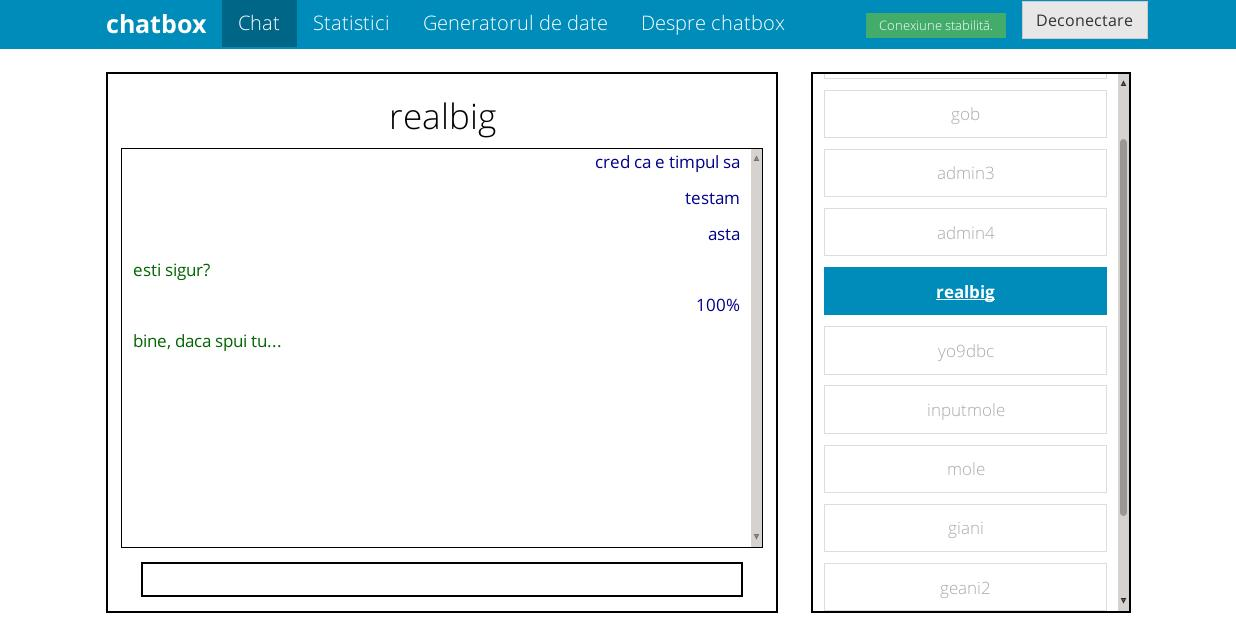
\includegraphics[width=150mm]{img/over.jpg}
\caption{Interfata modulului de mesagerie \label{overflow}}
\end{figure}

\vspace{3mm}
Inspiratie pentru acest proiect sunt serviciile de mesagerie instantanee 
precum \textit{Y!Messenger}, \textit{Google Talk} sau 
\textit{Facebook Messenger}, pentru a numi cateva.
\vfill

\begin{figure}[h!]
        \centering
        \begin{subfigure}[b]{0.45\textwidth}
                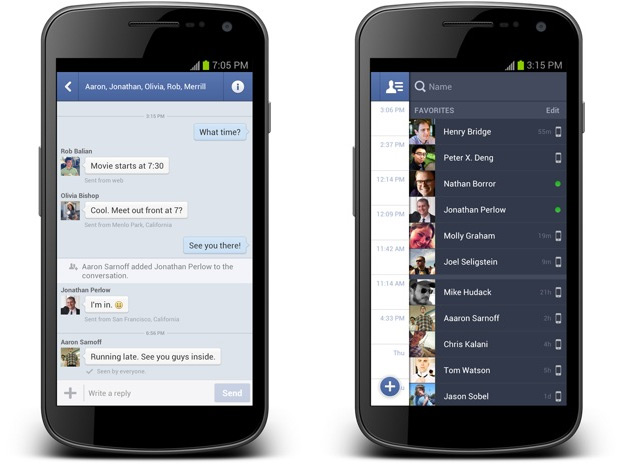
\includegraphics[height=5cm]{img/fb_mess.jpg}
                \caption{Facebook Messenger}
               % \label{fig:gull}
        \end{subfigure}%
        ~ \qquad 
        \begin{subfigure}[b]{0.45\textwidth}
                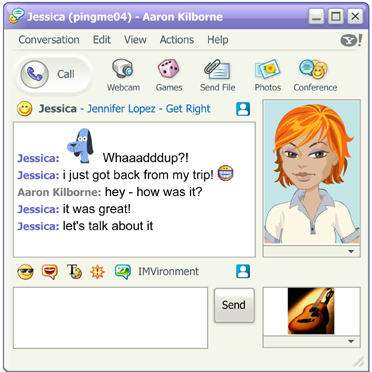
\includegraphics[height=5cm]{img/yahoo_mess.jpg}
                \caption{Yahoo! Messenger}
                %\label{fig:tiger}
        \end{subfigure}
        \caption{Servicii de mesagerie digitala}%\label{fig:animals}
\end{figure}



In prezent, \textbf{Chatbox} poate fi accesat la adresa
\textbf{penultim.ddns.net/chatbox}.



\newpage
\section{Resurse logice}
Resursele logice sunt componentele software ale calculatorului, care au functii de administrare a resurselor si a datelor.

In cazul proiectului \textbf{Chatbox}, acestea reprezinta mijlocul prin care
pagina web este programata, monitorizata si administrata.

\subsection{Sistemul MySQL}
MySQL\cite{mysql} este cel mai folosit SGBD\citep{sgbd} open-source, 
la ora actuala. Produs initial de compania suedeza MySQL AB 
și distribuit sub Licența Publică Generală GNU\cite{free}, 
in prezent MySQL este dezvoltat
de Corporatia Oracle.

Ca instrument de management pentru bazele de date MySQL
este folosita o aplicatie PHP numita phpMyAdmin.

\subsection{Limbajul PHP}
Limbajul de programare PHP\citep{php} este folosit pe scară largă 
în dezvoltarea paginilor și aplicațiilor web.

Se folosește în principal înglobat în codul HTML, dar poate fi 
utilizat si pentru programarea aplicatiilor CLI (linie de comanda).

PHP este disponibil sub Licenṭa PHP ṣi Free Software Foundation 
îl consideră a fi un software liber\citep{free}.

\subsubsection{Libraria PDO}
PHP Data Objects\citep{pdo} este o componenta PHP ce permite accesarea unor SGBD din
programe PHP. \textbf{Chatbox} foloseste in mod exclusiv componenta PDO pentru 
accesarea bazei de date. 

\subsubsection{Libraria Ratchet}
Websocket\citep{websocket} este un protocol ce furnizeaza o conexiune duplex prin o legatura TCP. Tehnologia Websocket a fost dezvoltata odata cu initiativa de 
inovare HTML5. 

Folosind tehnologia Websocket, se pot trimite date in timp real intre 
client si server. \textbf{Chatbox} foloseste acest protocol pentru
transmiterea instantanee a mesajelor si a datelor.

Ratchet\citep{ratchet} este o librarie ce permite utilizarea protocolului 
Websocket, in limbajul PHP.

\subsection{Limbajul JavaScript}
JavaScript (sau ECMAScript) este un limbaj de programare orientat pe obiecte\citep{javascript}, ce ruleaza in browserele utilizatorilor. 

Limbajul este binecunoscut pentru folosirea sa în construirea siturilor web. În ciuda numelui și a unor similarități în sintaxă, între JavaScript și limbajul Java nu există nicio legătură.

\subsubsection{Tehnica AJAX}
O tehnică de construire a paginilor web tot mai întâlnită în ultimul timp este AJAX, abreviere de la „Asynchronous JavaScript and XML”. Această tehnică constă în executarea de cereri HTTP în fundal, fără a reîncărca toată pagina web, și actualizarea numai anumitor porțiuni ale paginii.

\textbf{Chatbox} foloseste tehnica AJAX pentru a incarca o multitudine de
elemente, precum mesajele text primite sau lista de utilizatori activi. 

\subsubsection{Libraria jQuery}
jQuery\citep{jquery} este o platformă de dezvoltare JavaScript, concepută pentru a ușura și îmbunătăți procese precum traversarea arborelui DOM\citep{dom} în HTML, managementul evenimentelor, animații și cereri tip AJAX.

\subsubsection{Libraria chart.js}
Chart.js\cite{chartjs} este o librarie JavaScript ce permite afisarea 
unor grafice in mod dinamic. Graficele sunt redimensionate, la nevoie, dupa 
marimea ecranului clientului. 

Proiectul \textbf{Chatbox} foloseste chart.js pentru afisarea rezultatelor
numerice a unor interogari SQL si pentru vizualizarea de statistici.

\subsubsection{Libraria Bootstrap}
Bootstrap este cel mai popular framework de HTML, CSS, si JS dedicat dezvoltarii proiectelor Web. 

Bootstrap permite aranjarea elementelor grafice intr-un mod potrivit marimii ecranului vizitatorului. Astfel, site-ul va fi afisat satisfacator atat pe calculatoare Desktop, cat si pe tablete si telefoane.

\subsection{Limbajul Python}
Python este un limbaj de programare dinamic multi-paradigmă\cite{python}, creat în 1989 de programatorul olandez Guido van Rossum\cite{pythonWiki}.

Python pune accentul pe curățenia și simplitatea codului, iar sintaxa sa le permite dezvoltatorilor să exprime unele idei programatice într-o manieră cât mai clară și mai concisă.

Generatorul de date folosit de \textbf{Chatbox} este implementat in Python 3.

\subsection{Despre serverul Linux}
Codul proiectului \textbf{Chatbox} este rulat pe un calculator personal
 \textit{HP Compaq 6005 Pro}
care serveste, printre altele, drept server web. 
Sistemul are urmatoarele caracteristici:
\begin{itemize}
  \item Procesor: AMD Athlon II X2 2.8GHz
  \item Memorie: 2GB RAM DDR3
  \item Hard Drive: 2TB, Samsung
  \item Placa de retea: 100Mbps
  \item Sistem de operare: Debian 8
\end{itemize}

Pentru a dispune de o adresa permanenta a acestui server, 
am folosit serviciile de DNS dinamic ale firmei NoIP\cite{noip}.

\subsubsection{Sistemul de operare Debian 8}
Debian\cite{debian} este un sistem de operare compus din software liber\cite{free}, și o distribuție populară și foarte influentă între distribuțiile GNU/Linux.

Versiunea 8 a sistemului de operare este cunoscuta in prezent sub 
numele de \textit{testing}. Pachetele de software pentru versiunea 
\textit{testing} sunt, dupa cum sugereaza si numele, in curs de testare.
Totusi, sunt destul de stabile pentru modul in care 
este utilizat acest sistem.

\subsubsection{Serverul HTTP Apache 2}
Apache este un server HTTP open-source. Acesta reprezinta standardul in 
industria de web hosting, fiind cel mai folosit server HTTP, fiind folosit de 
53.34\% din site-urile web\cite{apache53}.

\subsubsection{Sistemul de monitorizare daemontools}
Daemontools\cite{daemon} este o colectie de unelte software folosite pentru 
controlul si monitorizarea serviciilor UNIX. 

Daemontools este folosit de \textbf{Chatbox} pentru a monitoriza serverul 
de \textit{websockets} si a-l reporni in eventualitatea unei erori.

\subsection{Procesorul \LaTeX}
Acest document a fost compus folosind sistemul \LaTeX  care permite prepararea
acestuia pentru tipărire în format electronic,
cu ajutorul limbajului de programare \TeX.

\newpage
\section{Descrierea proiectului}

\subsection{Baza de date}

\subsection{Sistemul de autentificare}

\subsection{Sistemul de mesagerie}

\subsubsection{Interfata}

\subsubsection{Serverul de websockets}

\subsection{Generarea si vizualizarea datelor}

\subsubsection{Generatorul de date}

\subsubsection{Vizualizarea datelor prin grafice}

\newpage
\section{Bibliografie}
\begingroup
\renewcommand{\section}[2]{}%
\begin{thebibliography}{99}

\bibitem{mysql} 
	MySQL \\
	http://www.mysql.com/about/
	
\bibitem{sgbd}
	Système de Gestion de Base de Données\\
	http://ro.wikipedia.org/wiki/Sistem\_de\_gestiune\_a\_bazelor\_de\_date

\bibitem{php}
	PHP Hypertext Processor\\
	http://php.net/manual/en/intro-whatis.php

\bibitem{pdo}
	PDO: PHP Data Objects\\
	http://php.net/manual/en/intro.pdo.php
	
\bibitem{websocket}
	Websocket\\
	https://www.websocket.org/
	
\bibitem{ratchet}
	Ratchet: a Websockets Library\\
	http://socketo.me/
	
\bibitem{javascript}
	Objects in Javascript\\
	http://www.w3.org/community/webed/wiki/Objects\_in\_JavaScript
	
\bibitem{jquery}
	jQuery: The Write Less, Do More, JavaScript Library\\
	https://jquery.com/
	
\bibitem{dom}
	Document Object Model
	http://www.w3.org/DOM/

\bibitem{chartjs}
	Chart.js: Open source HTML5 Charts \\
	http://www.chartjs.org/
	
\bibitem{bootstrap}
	Bootstrap -- Designed for everyone, everywhere \\
	http://getbootstrap.com/
	
\bibitem{python}
	Python \\
	https://www.python.org/about/

\bibitem{pythonWiki}
	Python, articol Wikipedia\\
	http://ro.wikipedia.org/wiki/Python
	
\bibitem{noip}
	No-IP: a Dynamic DNS company \\
	http://www.noip.com/
	
\bibitem{debian}
	Debian GNU/Linux \\
	https://www.debian.org/intro/about

\bibitem{free}
	Software liber / Free Software \\
	https://www.fsf.org/about/what-is-free-software
	
\bibitem{apache53}
	June 2013 Web Server Survey\\
http://news.netcraft.com/archives/2013/06/06/june-2013-web-server-survey-3.html
	
\bibitem{daemon}
	daemontools\\
	http://cr.yp.to/daemontools.html

\end{thebibliography}
\endgroup
\newpage
\tableofcontents

\end{document}